\documentclass[10pt,twocolumn]{article}
\usepackage[margin=0.75in]{geometry}
\usepackage[T1]{fontenc}
\usepackage[utf8]{inputenc}
\usepackage{lmodern}
\usepackage{microtype}
\usepackage{amsmath,amssymb,amsthm}
\usepackage{booktabs}
\usepackage{xcolor}
\usepackage{tikz}
\usetikzlibrary{positioning,arrows.meta,fit,calc}
\usepackage{pgfplots}
\pgfplotsset{compat=1.18}
\usepackage[ruled,vlined,linesnumbered]{algorithm2e}
\usepackage[colorlinks,linkcolor=blue!50!black,citecolor=blue!50!black,urlcolor=blue!50!black]{hyperref}
\usepackage[capitalise,noabbrev]{cleveref}

\newtheorem{proposition}{Proposition}
\newtheorem{definition}{Definition}
\newcommand{\todo}[1]{\textcolor{red!70!black}{[\textbf{TODO:} #1]}}
\newcommand{\Gt}{G_t}

\title{Defending Attack Graphs That Move:\\
Telemetry-Driven Exposure, Incremental Shortest Paths,\\
and Joint Detection--Deception Placement\\[4pt]
\large Internal draft v0 --- not for distribution}
\author{Lucas Sotomayor\\BASE4 Security, R\&D+i}
\date{November 4, 2026}

\begin{document}
\maketitle

\begin{abstract}
Attack-graph defenses for Active Directory (AD) are computed on snapshots, yet the
edges that matter most---interactive sessions, local-admin grants, ACL changes---appear
and expire within hours. We describe a program that treats the attack graph as a
time-indexed state $\Gt$ maintained from security telemetry, and three components
built on it. (i)~A deterministic, idempotent \emph{projection rule} that maps OCSF
provenance events to attack-graph edge changes, with a conformance suite of 17
cases; writing it surfaced two defects in a production parser that we fixed.
(ii)~An \emph{incremental oracle} that maintains shortest distances from every node
to every crown jewel under edge insertions, deletions and weight changes, with a
work-based fallback to full recomputation. On a synthetic AD graph with 4.6k nodes
and 354k edges, frequent changes (sessions, admin grants) are repaired in
0.02--0.16\,ms on average against 310\,ms for recomputation; the worst case stays
within 1.1$\times$ of recomputation. (iii)~A \emph{joint detection--deception}
model that places detection rules on edges and traps on nodes under a per-path
detection guarantee, obtained by a node-splitting reduction that makes traps ordinary
rules for an existing exact MILP; it matches brute force on 100 instances with and
without a trap budget. On 20 synthetic instances, two traps lower the median cost of
a $\delta=0.05$ guarantee to 11\% of the rules-only optimum and raise feasibility from
6/20 to 18/20. All results are preliminary: synthetic catalogs, synthetic detection
rates and no large real AD.
\end{abstract}

\section{Introduction}

Defensive analyses of AD attack graphs, from BloodHound path queries~\cite{bloodhound}
to edge blocking~\cite{guo2022practical,guo2023scalable} and honeypot
placement~\cite{ngo2024catch}, take a collection snapshot as input. Two observations
motivate this work. First, the edges that create short paths to Domain Admin are
largely \emph{transient}: a privileged user logging on to a workstation creates a
\texttt{HasSession} edge that lasts as long as the credentials stay in memory. A
snapshot taken on Monday says little about Thursday. Second, the telemetry that
reveals those edges is already collected by the SOC---Windows 4624/4688, Sentinel,
EDR---but it lives in a different graph: a provenance graph of what happened, not an
attack graph of what could happen.

We connect the two. The attack graph becomes a state $\Gt$ updated by events, and
every defensive question becomes a query or an optimisation over $\Gt$.

\paragraph{Contributions.}
\begin{itemize}
\item A two-layer model of $\Gt$ and a \textbf{projection rule} from OCSF provenance
events to attack-graph changes, with explicit edge support, idempotent deltas,
watermark-based expiry and identity resolution that refuses to guess
(\cref{sec:projection}). A reference implementation passes a 17-case conformance
suite shared with the production engine.
\item An \textbf{incremental distance oracle} for crown-jewel exposure in the style of
Ramalingam--Reps~\cite{ramalingam1996incremental}, with a fallback triggered by the
\emph{edge work} of the affected subtree rather than its size, which matters with group
hubs (\cref{sec:oracle}).
\item A \textbf{joint detection--deception} formulation: a reduction that turns node
traps into edge rules, so that one exact MILP chooses detection rules and traps under a
per-path guarantee, plus a trap budget (\cref{sec:joint}).
\item An evaluation of the three components on GOADv2~\cite{goad,bhsample} and synthetic
AD graphs (\cref{sec:eval}), with every result verified against an independent
reference (brute force or full Dijkstra).
\end{itemize}

\section{Background and related work}\label{sec:related}

\paragraph{Attack graphs and hardening.} Attack graphs were formalised by Jha et
al.~\cite{jha2002two}; minimum-cost hardening~\cite{wang2006hardening} and IDS sensor
placement~\cite{noel2008sensor} are early optimisation uses. For AD, Guo et al.\ study
edge blocking with fixed-parameter~\cite{guo2022practical} and scalable
algorithms~\cite{guo2023scalable}, and Goel et al.\ combine a neural dynamic program
with evolutionary search~\cite{goel2022defending}.

\paragraph{Interdiction and security games.} Shortest-path network
interdiction~\cite{israeli2002interdiction} and its stochastic variants~\cite{morton2007models}
are the operations-research root of our defender. Double-oracle methods solve
zero-sum security games on graphs~\cite{jain2011double}. Alert triage as a game is
studied by Schlenker et al.~\cite{schlenker2017alerts}. Arc interdiction combined with
monitoring appears in Nguyen, Song and Smith~\todo{full reference, Networks 2023}.

\paragraph{Deception.} Honeypot allocation over attack graphs~\cite{anwar2020honeypot},
the survey by Pawlick et al.~\cite{pawlick2019taxonomy}, and honeypot placement in
dynamic AD graphs~\cite{ngo2024catch} are closest to our trap model. Ngo et al.\ also
treat the graph as dynamic, but the dynamics are a model of the attacker's moves, not a
stream of observed telemetry.

\paragraph{Dynamic shortest paths.} Incremental single-source shortest paths go back
to Ramalingam and Reps~\cite{ramalingam1996incremental}; LPA*~\cite{koenig2004lpa} is the
planning variant; Demetrescu and Italiano~\cite{demetrescu2004apsp} give fully dynamic
all-pairs bounds. We use the simplest of these ideas and show where it pays off on AD
graphs and where it does not.

\paragraph{Telemetry schemas.} OCSF~\cite{ocsf} is the event schema of the projection;
detection content is mapped to ATT\&CK techniques, whose use in EDR products was
measured by Virkud et al.~\cite{virkud2024edr}.

\section{The state $\Gt$}\label{sec:model}

\begin{definition}[Two-layer state]
$\Gt=(V_t,\;E^{\mathrm{atk}}_t\cup E^{\mathrm{prov}}_t,\;w_t,\;q_t,\;r)$. Attack edges
$(u,\kappa,v)\in E^{\mathrm{atk}}_t$ mean ``controlling $u$ lets the attacker acquire
$v$'' with BloodHound semantics and directions~\cite{bloodhound}: \texttt{HasSession}
goes from host to user, \texttt{AdminTo} and \texttt{CanRDP} from principal to host.
Provenance edges are timestamped OCSF events. $q_t$ are detection probabilities on edges
(rules) or nodes (traps), $w_t$ are attack-edge weights and $r$ node values.
\end{definition}

Each attack edge carries its \emph{origins} (\texttt{snapshot}, \texttt{observed}), its
\emph{support} (the set of event ids sustaining it), first and last evidence times, an
expiry time and a confidence (\texttt{confirmed} if an event shows it exercised,
\texttt{inferred} if it is only enabled). An edge exists in $\Gt$ while it has the
snapshot origin, or a non-empty support and an unexpired expiry. This keeps both
sources of truth: the collector's snapshot and what telemetry has observed since.

\begin{figure}[t]
\centering
\resizebox{\columnwidth}{!}{%
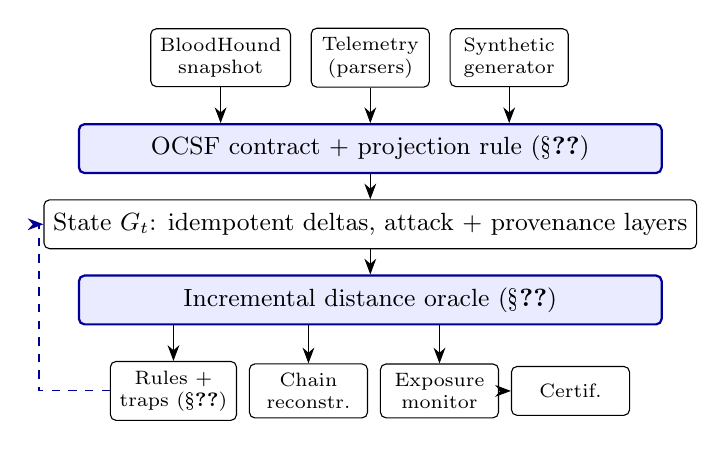
\begin{tikzpicture}[
  box/.style={draw, rounded corners=2pt, minimum width=7.4cm, minimum height=0.62cm, align=center, font=\small},
  new/.style={box, fill=blue!8, draw=blue!60!black, thick},
  small/.style={draw, rounded corners=2pt, minimum width=1.5cm, minimum height=0.62cm, align=center, font=\scriptsize},
  >={Stealth[length=2mm]}, node distance=0.32cm]
\node[small] (bh) {BloodHound\\snapshot};
\node[small, right=0.25cm of bh] (tel) {Telemetry\\(parsers)};
\node[small, right=0.25cm of tel] (sim) {Synthetic\\generator};
\node[new, below=0.45cm of tel] (proj) {OCSF contract + projection rule (\S\ref{sec:projection})};
\node[box, below=of proj] (state) {State $\Gt$: idempotent deltas, attack + provenance layers};
\node[new, below=of state] (orc) {Incremental distance oracle (\S\ref{sec:oracle})};
\node[small, below=0.45cm of orc, xshift=-2.5cm] (s1) {Rules +\\traps (\S\ref{sec:joint})};
\node[small, right=0.15cm of s1] (s2) {Chain\\reconstr.};
\node[small, right=0.15cm of s2] (s3) {Exposure\\monitor};
\node[small, right=0.15cm of s3] (s4) {Certif.};
\foreach \a in {bh,tel,sim} \draw[->] (\a) -- (\a |- proj.north);
\draw[->] (proj) -- (state); \draw[->] (state) -- (orc);
\foreach \a in {s1,s2,s3} \draw[->] (orc.south -| \a) -- (\a);
\draw[->] (s3) -- (s4);
\draw[->, dashed, blue!60!black] (s1.west) -- ++(-0.9,0) |- (state.west);
\end{tikzpicture}}
\caption{Architecture. Shaded components are new in this work. The dashed arrow is the
feedback loop: what the defender deploys enters $\Gt$ as deltas.}
\label{fig:arch}
\end{figure}

\section{Projection: provenance to attack edges}\label{sec:projection}

The projection is a pure, deterministic function from an OCSF envelope and an identity
table to a list of \texttt{AttackDelta}s: \textsc{Assert}(edge, event, confidence, ttl),
\textsc{Retract}(edge, event), \textsc{Close}(edge, at) and \textsc{Unresolved}(reason).
Deltas are keyed by event id, so replaying an envelope is a no-op; a tombstone retracts
the support its event contributed; a correction is a retract followed by re-projection.

\begin{table*}[t]
\centering\small
\caption{Projection rules v0. $lt$ is the OCSF \texttt{logon\_type\_id}, numbered as the
Windows 4624 LogonType for values 2--13.\todo{verify against the official OCSF 1.4 enum}}
\label{tab:rules}
\begin{tabular}{@{}lll@{}}
\toprule
Event & Condition & Output \\
\midrule
Auth.\ logon & success, $lt\in\{2,10,11,12\}$ & \texttt{HasSession}$(h{\to}u)$, confirmed \\
Auth.\ logon & success, $lt=10$ & also \texttt{CanRDP}$(u{\to}h)$ \\
Auth.\ logon & success, $lt\in\{4,5,9\}$ & \texttt{HasSession}, inferred \\
Auth.\ logon & $lt\in\{3,8\}$, failure, no $lt$ & nothing \\
Auth.\ logoff & session observed & \textsc{Close} with grace \\
Process launch & user not system/machine & \texttt{HasSession}, inferred, short ttl \\
Tombstone & --- & \textsc{Retract} its support \\
\bottomrule
\end{tabular}
\end{table*}

\paragraph{Design choices.} Interactive, remote-interactive and cached logons leave
reusable credentials on the host, so they are sessions in the BloodHound sense; network
logons (type~3) normally do not, and become \texttt{AdminTo} evidence only together with
privilege events that the engine does not parse yet. A logoff does not erase credentials
from memory immediately, so it closes the session after a grace period rather than
retracting it.

\paragraph{Time.} The time of an edge is the event time. An out-of-order event can lower
\emph{first seen} but never advances expiry, and expiry is driven by the stream watermark,
not the wall clock: reprocessing a historical day yields the same state as processing it
live.

\paragraph{Identity resolution.} Parsers name users \texttt{NETBIOS\textbackslash user}
and hosts by whatever the event carries; BloodHound uses UPN-like names, FQDNs and SIDs.
The rule uses the SID when present, otherwise normalises against the snapshot's domain
table and accepts a short host name only if exactly one FQDN matches. Otherwise it emits
\textsc{Unresolved}: a session on the wrong host invents an attack path, which is worse
than a missing one.

\paragraph{Defects found.} Specifying the rule against the production engine exposed six
prerequisites; two were defects. The OCSF projection dropped the logon type, and a failed
4625 parsed by the Sysmon/Security parser reached OCSF without a status---indistinguishable
from a successful logon---because that parser flagged failures with a field the projection
did not read. Both are fixed upstream with tests; the other four (logoff, privilege and
group-change events, SIDs, process host) are missing data, not errors.

\section{Incremental distance oracle}\label{sec:oracle}

For each terminal $t$ (a crown jewel), the oracle keeps $d_t(v)$, the shortest distance
from $v$ to $t$ under non-negative weights, and the next hop $\sigma_t(v)$. One structure
per terminal answers ``how close is any compromised node to $t$'', and distances between
terminals give the matrix that routing-style solvers need.

\begin{algorithm}[t]
\caption{Repair after deleting or raising edge $(u,v)$ for terminal $t$}\label{alg:raise}
\small
\If{$\sigma_t(u)\neq v$}{\Return \tcp*{not a tree edge}}
$A\gets\{u\}$; $W\gets\deg(u)$\;
\ForEach{$x$ popped from a stack started at $u$}{
  \ForEach{in-neighbour $p$ of $x$ with $\sigma_t(p)=x$, $p\notin A$}{
    $A\gets A\cup\{p\}$; $W\gets W+\deg(p)$\;
    \lIf{$W>\tau\,|E|$}{recompute $t$ from scratch; \Return}
  }
}
\lForEach{$x\in A$}{$d_t(x)\gets\min_{(x,y),\,y\notin A} w(x,y)+d_t(y)$}
run Dijkstra on the reverse graph restricted to $A$, seeded with those values\;
\end{algorithm}

Insertions and decreases propagate the improvement backwards with Dijkstra and touch
only nodes that improve. Deletions and increases (\cref{alg:raise}) do nothing unless
the edge is in the shortest-path tree; otherwise only the subtree $A$ of nodes whose path
went through it is reset, seeded from the unaffected frontier, and repaired.

\begin{proposition}
After \cref{alg:raise}, $d_t$ equals the shortest distances in the updated graph.
\end{proposition}
\begin{proof}[Sketch]
A node outside $A$ keeps a tree path to $t$ that avoids $(u,v)$; its length is unchanged
and, since the update only removes options, no shorter path appeared. Nodes in $A$ are
recomputed by Dijkstra from correct boundary values, which is exact because every
shortest path from $x\in A$ leaves $A$ at its first node outside $A$.
\end{proof}

\paragraph{Work-based fallback.} The first version fell back to recomputation when $|A|$
exceeded a fraction of $|V|$. On AD graphs with expanded groups this was the wrong
measure: a few hundred nodes can carry hundreds of thousands of edges, and local repair
became slower than recomputation. The fallback now counts the in- and out-degree of the
nodes added to $A$ and stops as soon as it exceeds $\tau|E|$ ($\tau=0.1$).

\paragraph{What-if.} \texttt{what\_if(changes)} applies a batch, yields, and restores the
previous weights; selection loops that price one candidate rule or trap at a time use it.

\section{Joint detection and deception}\label{sec:joint}

\paragraph{Detection guarantee.} Following detcover~\cite{detcover}, a rule $r$ covers the edges whose
ATT\&CK technique and telemetry scope it observes, fires with probability $q_r$ and costs
$c_r$ expected false positives per day. Under independence, the probability that a path
$P$ evades the active rules $x$ is $\prod_{e\in P}\prod_{r\ni e}(1-q_r)^{x_r}$, so
requiring every source--terminal path to be detected with probability at least $1-\delta$
is linear in $x$ through potentials:
\begin{align*}
\min\ & \textstyle\sum_r c_r x_r\\
\text{s.t. } & \pi_v-\pi_u-\textstyle\sum_{r\ni e} w_r x_r\le 0 \quad \forall e=(u,v),\\
& \pi_s=0,\ \pi_t\ge\theta,\ 0\le\pi\le\theta,\ x\in\{0,1\}^R,
\end{align*}
with $w_r=-\log(1-q_r)$ and $\theta=-\log\delta$. The same codebase solves a variant with
edge blocking, a randomised triage defender against an informed attacker (Stackelberg),
and a lazy constraint-generation version for large graphs.

\paragraph{Traps as rules.} PERIPLO~\cite{periplo} places traps on nodes: acquiring a trapped node is
detected with certainty. We split every trap candidate $v$ (never the source or a
terminal) into $v\to v^{\#}$, redirect $v$'s out-edges to leave from $v^{\#}$, and add a
rule \texttt{trap:}$v$ with $q=1$ that covers only the new edge.

\begin{proposition}
For any choice of rules $R'$ and traps $T'$, the minimum evasion weight from $s$ to the
terminals in the split instance with rules $R'\cup\{\texttt{trap:}v: v\in T'\}$ equals the
one in the original instance with rules $R'$ on edges and traps $T'$ on nodes.
\end{proposition}
\begin{proof}[Sketch]
Paths are in bijection: a path that continues from $v$ must traverse $v\to v^{\#}$, which
carries exactly the trap weight when $v\in T'$ and zero otherwise; edge weights of
redirected edges are unchanged because coverage depends only on technique and scope.
Terminals are not split, and a path that ends at $v$ is not a source--terminal path.
\end{proof}

Consequently every detcover solver chooses rules and traps jointly without modification. A
trap budget, as in PERIPLO, is one extra row $\sum_v x_{\texttt{trap:}v}\le k$.

\paragraph{Scope of the equivalence.} detcover's attacker wants to reach a terminal, so a
trap matters only on transit nodes. PERIPLO's attacker collects value per node under a time
budget and a pivot-switch cost; a trap on a dead-end node matters to it and not to this
reduction. Evaluating joint solutions against PERIPLO's attacker is future work.

\section{Evaluation}\label{sec:eval}

Everything runs in Python on one core of a shared cloud VM; times are single runs and vary
between runs by up to $\sim$1.5$\times$ for full recomputation. Code and data live in the
Graph Hunter repository~\cite{graphhunter} under \texttt{research/} (private branch).

\subsection{Projection}

The reference implementation passes the 17 conformance cases (all rules, idempotence,
out-of-order arrival, tombstones, corrections, ambiguous hosts and unknown domains). The
same JSON file is the target for the Rust implementation. The parser and schema fix adds
four tests; 57 tests of the canonical crate and 1{,}033 of the core engine pass.

\subsection{Oracle}

\paragraph{Correctness.} After every change, distances and paths are compared with a full
Dijkstra: 4{,}800 random changes on 30-node graphs (with and without the fallback),
5$\times$200 on GOADv2 and 150 on a synthetic AD graph with hubs. Disabling the repair of
increases on purpose makes the tests fail.

\begin{table}[t]
\centering\small
\caption{Oracle on a synthetic AD graph (\texttt{adgen}, scale 2000): 4{,}583 nodes,
353{,}526 edges, 4 terminals. Full recomputation for the 4 terminals: 310\,ms. Each change
is measured and then undone; ``fallbacks'' counts recomputations from scratch.}
\label{tab:oracle}
\footnotesize\setlength{\tabcolsep}{4pt}
\begin{tabular}{@{}lrrrr@{}}
\toprule
Change & mean (ms) & worst (ms) & fallbacks & speed-up \\
\midrule
New session & 0.025 & 0.36 & 0 & 12{,}557$\times$ \\
Session expires & 0.161 & 2.27 & 0 & 1{,}924$\times$ \\
AdminTo removed & 0.024 & 0.48 & 0 & 12{,}782$\times$ \\
ACL removed & 2.31 & 226 & 3 & 134$\times$ \\
Tree edge near $t$ & 20.2 & 346 & 21 & 15$\times$ \\
\bottomrule
\end{tabular}
\end{table}

\paragraph{Cost.} \Cref{tab:oracle} reports the graph whose group expansion creates hubs.
Frequent changes cost thousands of times less than recomputation because most of them do
not touch any shortest-path tree. The adversarial case, removing a tree edge next to a
terminal, averages 15$\times$ faster and its worst case (346\,ms) stays within
1.1$\times$ of recomputation thanks to the work-based fallback; before the fallback was
changed, local repair exceeded recomputation. On a sparser random AD-like graph (62{,}855
nodes, 132{,}507 edges) the mean repair is 0.016\,ms against 199\,ms per terminal for
recomputation. GOADv2 (46 nodes, 259 edges) is too small to say anything about scale; all
its changes take under 0.14\,ms.

\subsection{Joint detection and deception}

\paragraph{Exactness.} On 25 random instances (9 nodes, 5 rules, 3 trap candidates) the
MILP optimum on the split instance equals a brute force over rules and node traps that
does not use the reduction; the cases include optima with traps (8), without (7), and
infeasible instances (10). With a budget $k\in\{0,1,2\}$ the same holds on 75 more
instances. For random choices of rules and traps, evasion distances coincide.

\begin{figure}[t]
\centering
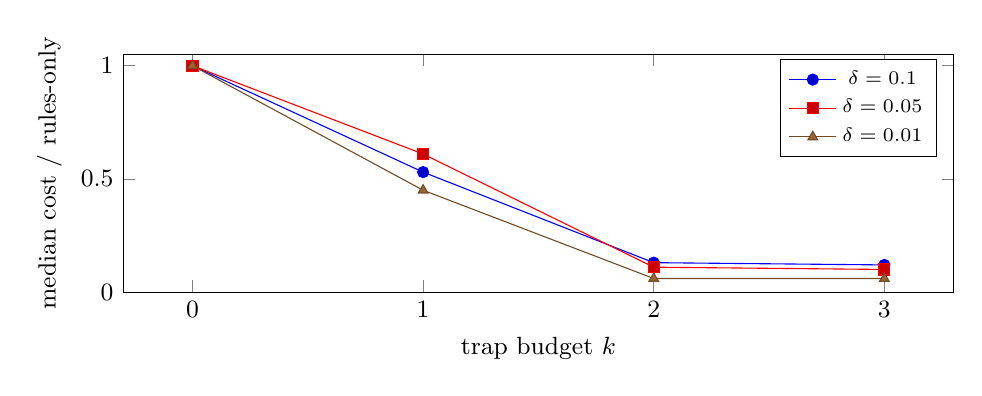
\begin{tikzpicture}
\begin{axis}[width=\columnwidth, height=4.6cm, xlabel={trap budget $k$},
  ylabel={median cost / rules-only}, xtick={0,1,2,3}, ymin=0, ymax=1.05,
  legend style={font=\scriptsize, at={(0.98,0.98)}, anchor=north east}, tick label style={font=\small},
  label style={font=\small}]
\addplot+[mark=*] coordinates {(0,1.00) (1,0.53) (2,0.13) (3,0.12)};
\addplot+[mark=square*] coordinates {(0,1.00) (1,0.61) (2,0.11) (3,0.10)};
\addplot+[mark=triangle*] coordinates {(0,1.00) (1,0.45) (2,0.06) (3,0.06)};
\legend{$\delta=0.1$, $\delta=0.05$, $\delta=0.01$}
\end{axis}
\end{tikzpicture}
\caption{Cost of the guarantee with up to $k$ traps (trap cost 5 FP/day-equivalent),
median over the instances feasible with rules only. 20 synthetic instances.}
\label{fig:traps}
\end{figure}

\begin{table}[t]
\centering\small
\caption{Feasible instances out of 20 (trap cost 5).}
\label{tab:feasible}
\begin{tabular}{@{}lrrrr@{}}
\toprule
$\delta$ & $k=0$ & $k=1$ & $k=2$ & $k=3$ \\
\midrule
0.10 & 12 & 17 & 18 & 18 \\
0.05 & 6 & 14 & 18 & 18 \\
0.01 & 1 & 7 & 12 & 17 \\
\bottomrule
\end{tabular}
\end{table}

\paragraph{Synthetic sweep.} On 20 instances of detcover's generator (121 nodes, about
340 edges, 25 rules with synthetic detection rates), the best evasion probability reachable
with all rules active has median 0.076, so rules alone cannot guarantee $\delta=0.05$ in 14
of 20 instances (\cref{tab:feasible}). Two traps restore feasibility in 18 of 20 and cut the
median cost to 11\% of the rules-only optimum where both exist (\cref{fig:traps}); at a trap
cost of 15 the reduction is to 25\%. Every MILP solves in under 0.2\,s.

\paragraph{GOADv2.} Using as footholds the users PERIPLO classifies as unprivileged, the best
evasion probability with every rule of the (synthetic) catalog is 0.12 in ESSOS, 0.33 in
NORTH and 0.54 in SEVENKINGDOMS. One trap on a transit user or computer gives the
$\delta=0.05$ guarantee in ESSOS and NORTH; in SEVENKINGDOMS the six admissible trap
candidates do not suffice. With detcover's default of 20 random footholds, GOAD's small
domains include accounts that are already Domain Admins and every instance is infeasible.

\section{Discussion and limitations}\label{sec:limits}

\begin{itemize}
\item \textbf{Traps are perfect by assumption.} The reduction inherits PERIPLO's $q=1$; one
trap then dominates any number of imperfect rules. A realistic trap model needs an
interaction probability, which the reduction already supports through the rule's $q$.
\item \textbf{Synthetic detection content.} Catalogs and detection rates are synthetic;
detcover already imports Sigma rules, which is the next step.
\item \textbf{Independence.} The linear guarantee assumes independent firings; detcover
quantifies the effect of common-cause correlation separately.
\item \textbf{No large real AD.} GOADv2 is small; client collections cannot enter the
repository. The worst case of the oracle on real hubs is measured only on a synthetic
generator.
\item \textbf{Projection parameters.} Session lifetimes and grace periods are uncalibrated
defaults; four prerequisites remain open (logoff, privilege and group-change events, SIDs,
process host).
\end{itemize}

\section{Roadmap}

(1)~Implement the projection in the Rust engine against the same conformance file.
(2)~Evaluate joint solutions against PERIPLO's value-collecting attacker and its exact
best response, and unify the certificate formats of the solvers. (3)~Calibrate edge
weights from attack chains reconstructed by the engine's Steiner-arborescence module, closing
the loop from observed intrusions to model parameters. (4)~Measure the oracle and the joint
model on a large real collection under the appropriate data agreements.

\section*{Items to verify before submission}
\begin{itemize}
\item Full reference for Nguyen, Song and Smith (Networks, 2023).
\item OCSF 1.4 \texttt{logon\_type\_id} values (checked only against a secondary source).
\item Page range of~\cite{jain2011double}: the two source bibliographies disagree
(305--312 vs 327--334).
\item Ramalingam--Reps, LPA* and Demetrescu--Italiano entries were written from memory.
\end{itemize}

\bibliographystyle{plain}
\bibliography{refs}
\end{document}
